\documentclass[tikz,border=3.14mm]{standalone}
\usepackage{amsmath}
\begin{document}
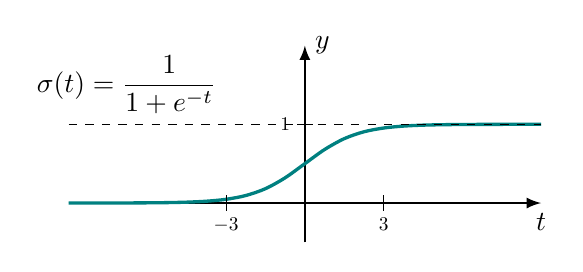
\begin{tikzpicture}
    \node[left] at (-1, 1.5) {$\sigma (t) = \dfrac{1}{1+e^{-t}}$};
    \draw[thick, -latex](-3, 0) -- (3, 0) node[below] {$t$};
    \draw[thick, -latex](0, -0.5) -- (0, 2) node[right] {$y$};
    \draw[very thick, teal, domain=-3:3,smooth,variable=\t] plot ({\t}, {1/(1+exp(-3*\t))});
    \draw[] (-1,0.1) -- (-1, -0.1) node [below, scale=0.7] {$-3$};
    \draw[] (1,0.1) -- (1, -0.1) node [below, scale=0.7] {$3$};
    \draw[] (0.1, 1) -- (-0.1, 1) node [left, scale=0.7] {$1$};
    \draw[dashed] (-3, 1) -- (3, 1);
 
\end{tikzpicture}
\end{document}